\section{Introduction}
This project is about the creation of a \textit{Miosix} driver for the ultrasonic distance sensor HCSR04 using hardware timers. 
\subsection{Problem statement}
The sensor HCSR04 is one of most used ultrasonic distance sensor in DIY project due to its low retail price. Moreover it has features that make it a good alternative for simple projects, some of its characteristics are:
\begin{itemize}
\item 0,02m-4m range;
\item 0.3 cm resolution;
\item quiescent current <2mA;
\item working current ~15mA.
\end{itemize}  
The aim of this project is to develop a driver for \textit{Miosix} operating system to allow developers to interface easily with this sensor.
\subsection{Summary of the work}
The driver uses hardware timer input capture mode to convert sensor answer into number representing the distance. The work was divided in two main phases:
\begin{enumerate}
\item Understand how hardware timers work and how to use inpute capture to convert sensor answer;
\item Actually implement the driver for \textit{Miosix} operating system.
\end{enumerate}

\pagebreak

\section{Design and implementation}
\subsection{How the sensor HCSR04 works}
\begin{minipage}{0.5\textwidth}
The sensor has 4 pins:
\begin{itemize}
\item VCC: 5V Supply; 
\item TRIGGER: Trigger Pulse Input;
\item ECHO: Echo Pulse Output;
\item GND: 0V Ground.
\end{itemize} 
\end{minipage}
\begin{minipage}{0.4\textwidth}
\begin{figure}[H]
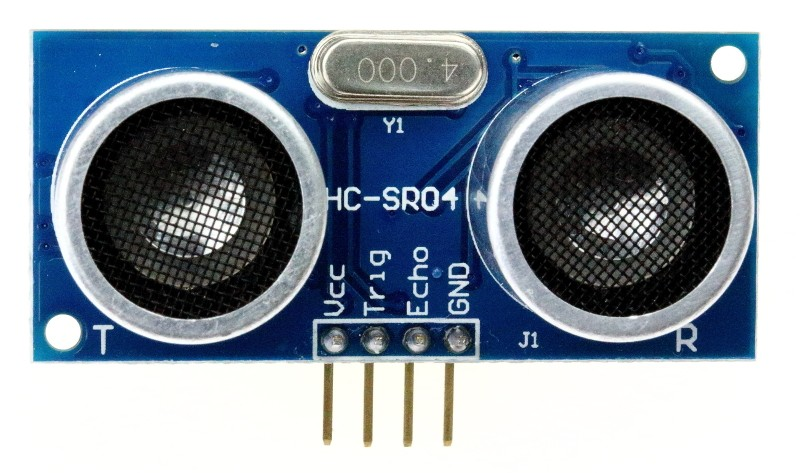
\includegraphics[width=\textwidth]{figures/raster/HCSR04}
\caption{\label{fig:sensor} HCSR04 sensor}
\end{figure}


\end{minipage} \hfill \\[1cm]



The basic principle of work consist of these steps:
\begin{enumerate}
\item Drive high level signal to TRIGGER pin for at least 10us;
\item The module sends eight sound burst  at 40 kHz and detect whether there is a
pulse signal back;
\item The module drive the ECHO pin to high level signal for as much microseconds as the time the sound wave has traveled. 
\end{enumerate} 
\subsection{Class design}
\subsection{Class implementation}


\section{Experimental evaluation}


\subsection{Experimental setup}
\subsubsection{Hardware setup}
\subsubsection{Software setup}
\subsection{Tests}
\subsection{Results}

\section{Conclusions and Future Works}

